\section{Frontend Implementierung}
\setauthor{Jonas Dorfinger}

Die Anforderungen an das Frontend sind sehr vielseitig, einerseits soll es wie eine Präsentation mit mehreren Slides aufgebaut,
andererseits soll das gesamte Projekt leicht wartbar und individualisierbar bleiben.
Die Daten werden dynamisch aus einem Konfigurationsfile ausgelesen, welches durch einen eigenen Generator generiert werden kann.

Um die UserExperience zu verbessern, wird auch auf wichtigen Dinge wie Angular Routing oder angemessenes styling Wert gelegt.
Nicht zu vernachlässigen ist dabei, der Fakt, dass webmap interaktiv sein soll.
Das bedeutet, dass der Userin oder dem User die Möglichkeit geboten werden soll, durch Slider oder true/false Switches
die Darstellung der aktuellen Daten auf der Page zu manipulieren.


\cleardoublepage

\subsection{Konfigurationsfile}
Das Konfigurationsfile ist ein JSON File, welches festlegt welche Slides (Pages) existieren, aber auch die zu darstellenden Daten definiert.
Hinweis: Grafische Darstellungen der Konfiguration sind weiter unten, bei anderen Kapiteln angeführt.

\begin{lstlisting}[label={lst:config.json}]{config.json}
{
  "name": "webmap showcase",
  "description": "this config is made to show how webmap configs look like",
  "pages": [
    {
      "title": "Bersbuch",
      "subtitle": "Anreise Dauer zum Bahnhof Bersbuch.",
      "description": [
        "Bersbuch ist ein Dorf in der Gemeinde Andelsbuch im Bregenzerwald."
      ],
      "mapOptions": {
        "zoom": 13,
        "center": [
          47.40198749647868,
          9.861946105957031
        ]
      },
      "datasources": [
        {
          "options": {},
          "id": "bersbuch-walk"
        }
      ],
      "controls": {
        "filters": [
          {
            "name": "Anreise Dauer Rad",
            "type": "slider",
            "dataSource": "bersbuch-bike",
            "unit": "Sekunden",
            "filterValue": "time"
          }
        ]
      }
    }
  ],
  "datasources": [
    {
      "options": {},
      "data": "bersbuch_walk.json",
      "id": "bersbuch_walk",
      "colorScheme": "my-color-scheme",
      "colorSchemeOrderValue": "time",
      "tooltip": [
        {
          "type": "value",
          "name": "time"
        },
        {
          "type": "text",
          "content": " Sekunden"
        }
      ]
    }
  ],
  "customColorSchemes": [
    {
      "id": "my-color-scheme",
      "colors": [
        "#f6d2a9",
        "#f5b78e",
        "#f19c7c",
        "#ea8171",
        "#dd686c",
        "#ca5268",
        "#b13f64"
      ]
    }
  ]
}
\end{lstlisting}

\subsubsection{Allgemeine Properties}
\textbf{Name}
Verleiht der ganzen Seite einen Namen.
Wird aktuell nicht angezeigt, kann aber durch Individualisierungen verwendet werden.

\textbf{Description}
Beschreibt die erzeugte Website etwas genauer.
Wird aktuell nicht angezeigt, kann aber durch Individualisierungen verwendet werden.

\subsubsection{Pages}
\emph{Pages} ist ein Array, welches die Ansichten definiert.
Jedes Element im Array, hat eine eigenen Map Ansicht, sowie eigene Daten, welche in der Sidebar angezeigt werden.

\textbf{Title}
Der Title ist der Name der Seite und wird groß hervorgehoben angezeigt.

\textbf{Subtitle}
Der Subtitle beschreibt in wenigen Wörtern, etwas genauer worum es bei der ausgewählten Karte geht.

\textbf{Description}
Description ist in diesem Fall ein Array von Strings, das bedeutet, es können mehrere Texteinträge angeführt werden,
was wiederrum einen Designtechnischen Grund hat.
Für jeden Eintrag wird ein eigener Absatz in der Sidebar generiert.

\textbf{Map Options}
Hier können in einem freien JSON Feld \href{https://leafletjs.com/SlavaUkraini/reference.html#map-option}{Leaflet-Map-Options}
übergeben werden, um die Darstellung der Map gezielt zu verändern.
Ein häufiger Anwendungsfall dafür ist es, den Ausrichtungspunkt zu ändern, um automatisch den richtigen Kartenausschnitt präsentiert zu bekommen.

\textbf{Data Sources}
Bei dem Array \emph{Data Sources} können Geo-Daten eingebunden werden, weiter unten werden diese Global definiert und hier
können diese referenziert werden.
Zusätzlich können wieder \emph{options}, in Form von einem JSON Objekt übergeben werden.

\textbf{Controls}
Hier können interaktive Elemente ausgewählt werden.
Es gibt vordefinierte Controls, aus denen man wählen kann.
Nach Absprache mit der triply, wurde entschieden, dass für diese Version ein Filter ausreichend ist.
Dieser Filter ist ein Slider, welcher auf eine bestimmte Property gebindet werden kann (\emph{filterValue}).
Mit dem Attribut \emph{dataSource} wird die zutreffende Data Source ausgewählt.
Zusätzlich kann noch eine Einheit (\emph{unit}) und auch ein Name für den Filter angegeben werden.

\subsubsection{Data Sources}
Ist ein Array welches mehrere Data Sources beinhalten kann.
Jedes JSON-Objekt hat mehrere Attribute die eine Data Source beschreiben.
Diese werden global definiert und können in jeder Page, auch mehrmals referenziert werden.

\textbf{ID}
Die ID wird benötigt, um eine Data Source referenzieren zu können, zum Beispiel bei der Erstellung von Pages.

\textbf{Data}
Data ist ein File-upload Feld, bei dem kann das Geo-JSON File hochgeladen werden, in welchem die Daten gespeichert sind.

\textbf{Options}
Hier können \href{https://leafletjs.com/SlavaUkraini/reference.html#map-option}{Leaflet-Map-Options} in einem freien JSON-Feld
übergeben werden, um die Art der Darstellung oder das Verhalten der Map zu verändern.

\textbf{Color Scheme}
Dieses Feld referenziert auf die ID eines Color Schemes, entweder man gibt den Namen eines
\href{https://carto.com/carto-colors/}{Carto-Color-Schemes} an oder man erstellt ein eigenes Custom-Color-Scheme.

\textbf{Color Scheme Order Value}
Um das Color-Scheme richtig anzuwenden, braucht man einen Value, um eine angemessene Skalierung zu berechnen, dieser Attributname
kann hier angegeben werden.

\textbf{Tooltip}
Der Tooltip ist ein Feature, welcher es ermöglicht Information beim hovern einer Data Source auf der Map anzuzeigen.
Es ist deshalb ein Array, damit man unbegrenzt viele Informationen angeben kann.
Jedes JSON-Objekt in diesem Array besitzt genau 2 Attribute, \emph{type} und \emph{name} oder \emph{content}.
Der \emph{type} gibt an, ob es sich um einen Value oder einen Text handelt, bei einem Value, muss der Attributname, des
Values bei dem anderen Attribute (\emph{Name}) angegeben werden.
Wird jedoch der Typ \emph{Text} ausgewählt, so muss lediglich ein String angegeben werden, welcher angezeigt wird (zum Beispiel
eine Einheit für den Value zuvor).

\subsubsection{Custom Color Schemes}
Hierbei handelt es sich um ein Array, in dem individuelle Color Schemes gespeichert werden können.
Wichtig, dass auch hier jedes JSON-Objekt eine ID erhält, um das Scheme referenzieren zu können.
Weiters befindet sich ein Array \emph{colors} in diesem Objekt, welches die HEX-Codes der Farben beinhaltet.

\subsection{Frontend Architektur und Aufbau}
Auf der linken Seite gibt, es eine Sidebar in der alle Informationen angezeigt werden, welche für die aktuell ausgewählte Seite relevant sind.
Auf der rechten Seite, wird die Map dargestellt, auf dieser werden die Data Sources angezeigt, sowie die Map-Options angewandt.
Die Services, verarbeiten und verteilen Daten zwischen den Components.

\begin{figure}[hbt!]
    \centering
    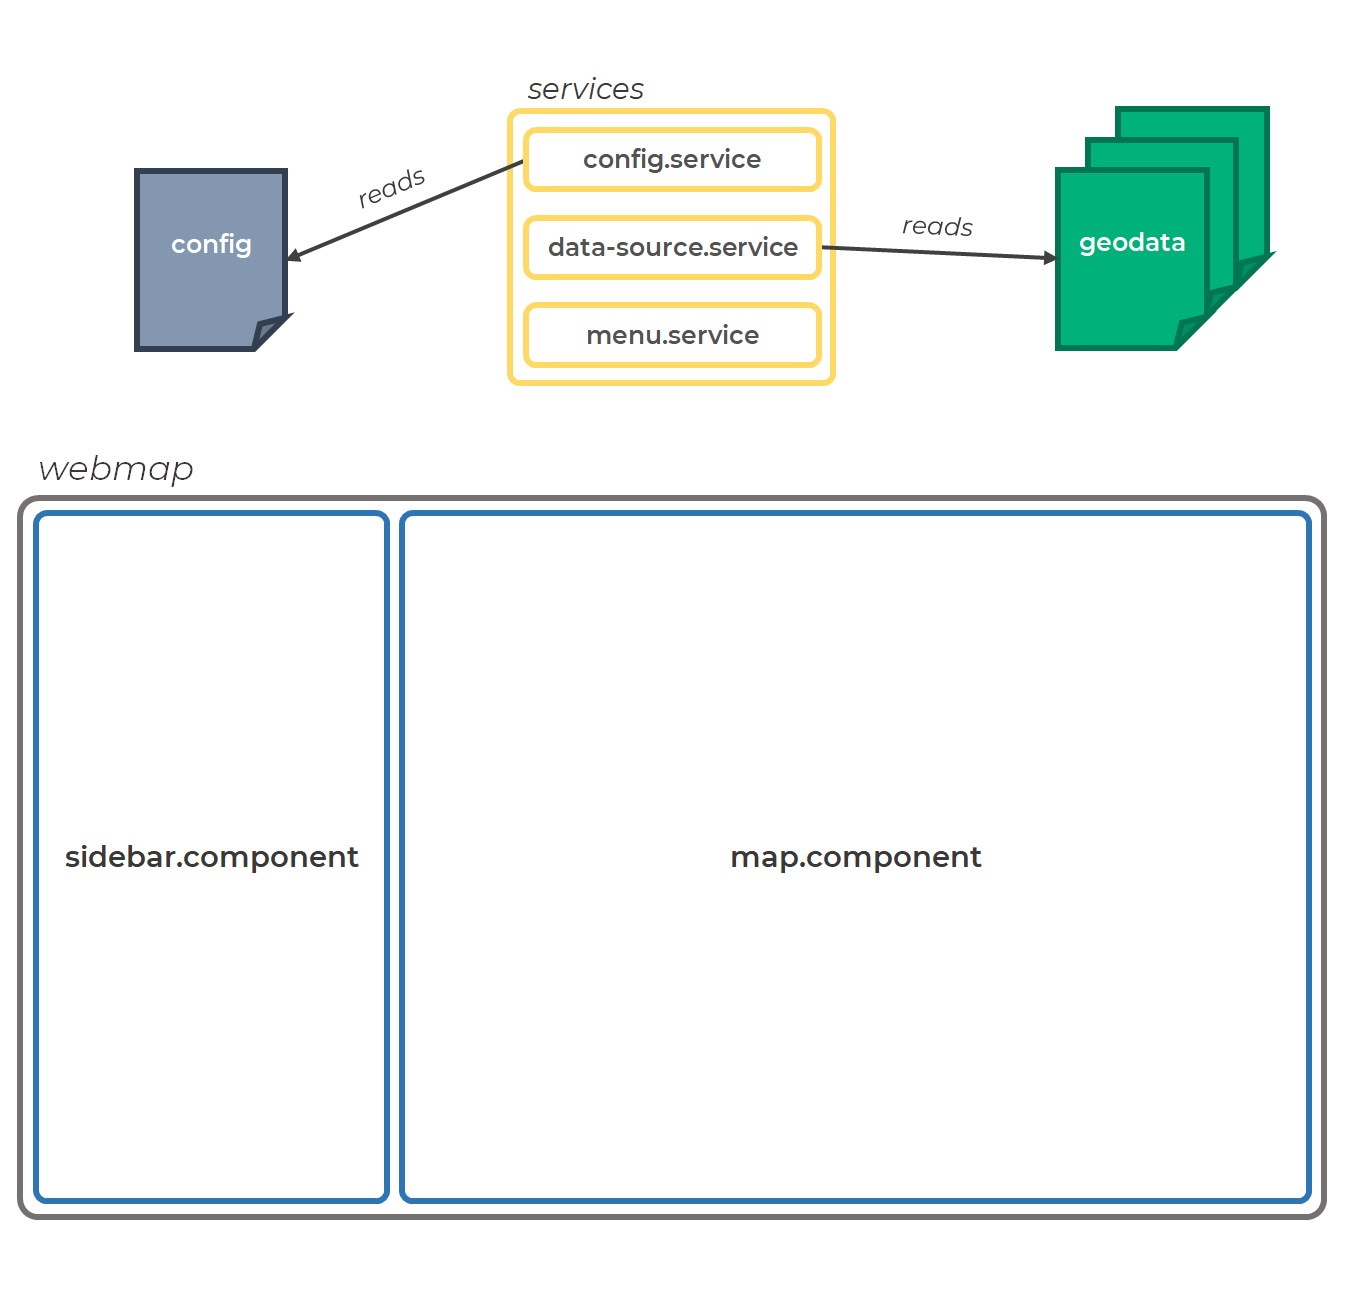
\includegraphics[scale=.6]{pics/frontend-architecture}
    \caption{Frontend Architektur}
    \label{fig:frontend-architecture}
\end{figure}

\cleardoublepage

\subsection{Services}
Services sind Angular ein spezielles Konstrukt zur Datenverarbeitung, der Hauptanwendungsfall ist der Austausch von Daten
zwischen mehreren Components.
Der große Vorteil dabei ist, diese Singletons sind, das bedeutet, es gibt genau eine Instanz für alle Komponenten, somit
ist es möglich, dass alle auf die gleichen Daten zugreifen.

\subsubsection{Config Service}
Der Config Service liest, das Konfigurationsfile aus bietet diesen Inhalt an andere Components an.
Über die App Component, wird die Konfiguration angefordert und weiterverarbeitet, so werden die Data Source Konfigurationsdaten
und die Custom Color Schemes herausgefiltert und an den ~\ref{subsubsec:data-source-service} weitergegeben.

\subsubsection{Data Source Service}
\label{subsubsec:data-source-service}
Das Ziel mit diesem Service ist es, einen globalen Pool an Data Sources zu erstellen, aus der jede Component jederzeit die
benötigten Data Sources anfordern und referenzieren kann, somit muss jede Data Source nur einmal erstellt werden und kann endlose Male weiterverwendet werden.

Jede Data Source besteht aus mehreren Layern, dadurch ist eine Data Source eine Leaflet \emph{LayerGroup}.
Der Service erhält zu Beginn die Informationen aus dem Konfigurationsfile, zuerst werden die Geo-Daten ausgelesen und entsprechend verarbeitet.
Es werden die verschiedenen Layer entsprechend der Daten erstellt und eingefärbt, wenn angegeben, wird hier auch der Tooltip zum Layer hinzugefügt.

Es werden alle \emph{Geometry Types} laut der \emph{GeoJSON Specification (RFC 7946)}~\cite{rfc7946} unterstützt:

\begin{itemize}
    \item Point
    \item LineString
    \item Polygon
    \item MultiPoint
    \item MultiLineString
    \item MultiPolygon
    \item \emph{GeometryCollection} ist nicht offiziell im Standard inkludiert, wird aber auch unterstützt.
    Diese Art von \emph{Geometry Types} kann mehrere andere \emph{Types} beinhalten.
\end{itemize}

\subsubsection{Menu Service}
Um die Navigation zu erleichtern, kann man mit den Pfeiltasten zwischen den Pages wechseln, aber auch ein globales Menü
steht zur Verfügung, um direkt zur gewünschten Page zu gelangen.
Dabei hat man eine kurze Übersicht über alle Pages und mit einem Klick auf die entsprechende Seite gelangt man auch dorthin.

\begin{figure}[hbt!]
    \centering
    
\includegraphics[scale=.9]{pics/menu}
    \caption{Menü zur Page Auswahl}
    \label{fig:menu}
\end{figure}

\subsection{Custom Color Schemes}
Color Schemes ermöglichen es, Bereiche auf Karten visuell besser darzustellen.
Es werden standardmäßig die Schemes der CartoColor Library verwendet, welche exzellente Schemes für Karten bereitstellt.
Ein Color Scheme besteht aus mehreren Farben, welche durch Abstufungen angeordnet sind (meistens von dunkel bis hell).
Auch bei den Individuellen Schemes ist dies nicht anders, es werden ein eindeutiger Name vergeben und HEX-Codes zugeordnet.

Der ~\ref{subsubsec:data-source-service} stellt sicher, dass alle Custom Color Schemes importiert und verwendet werden, wenn so konfiguriert.

\begin{figure}[hbt!]
    \centering
    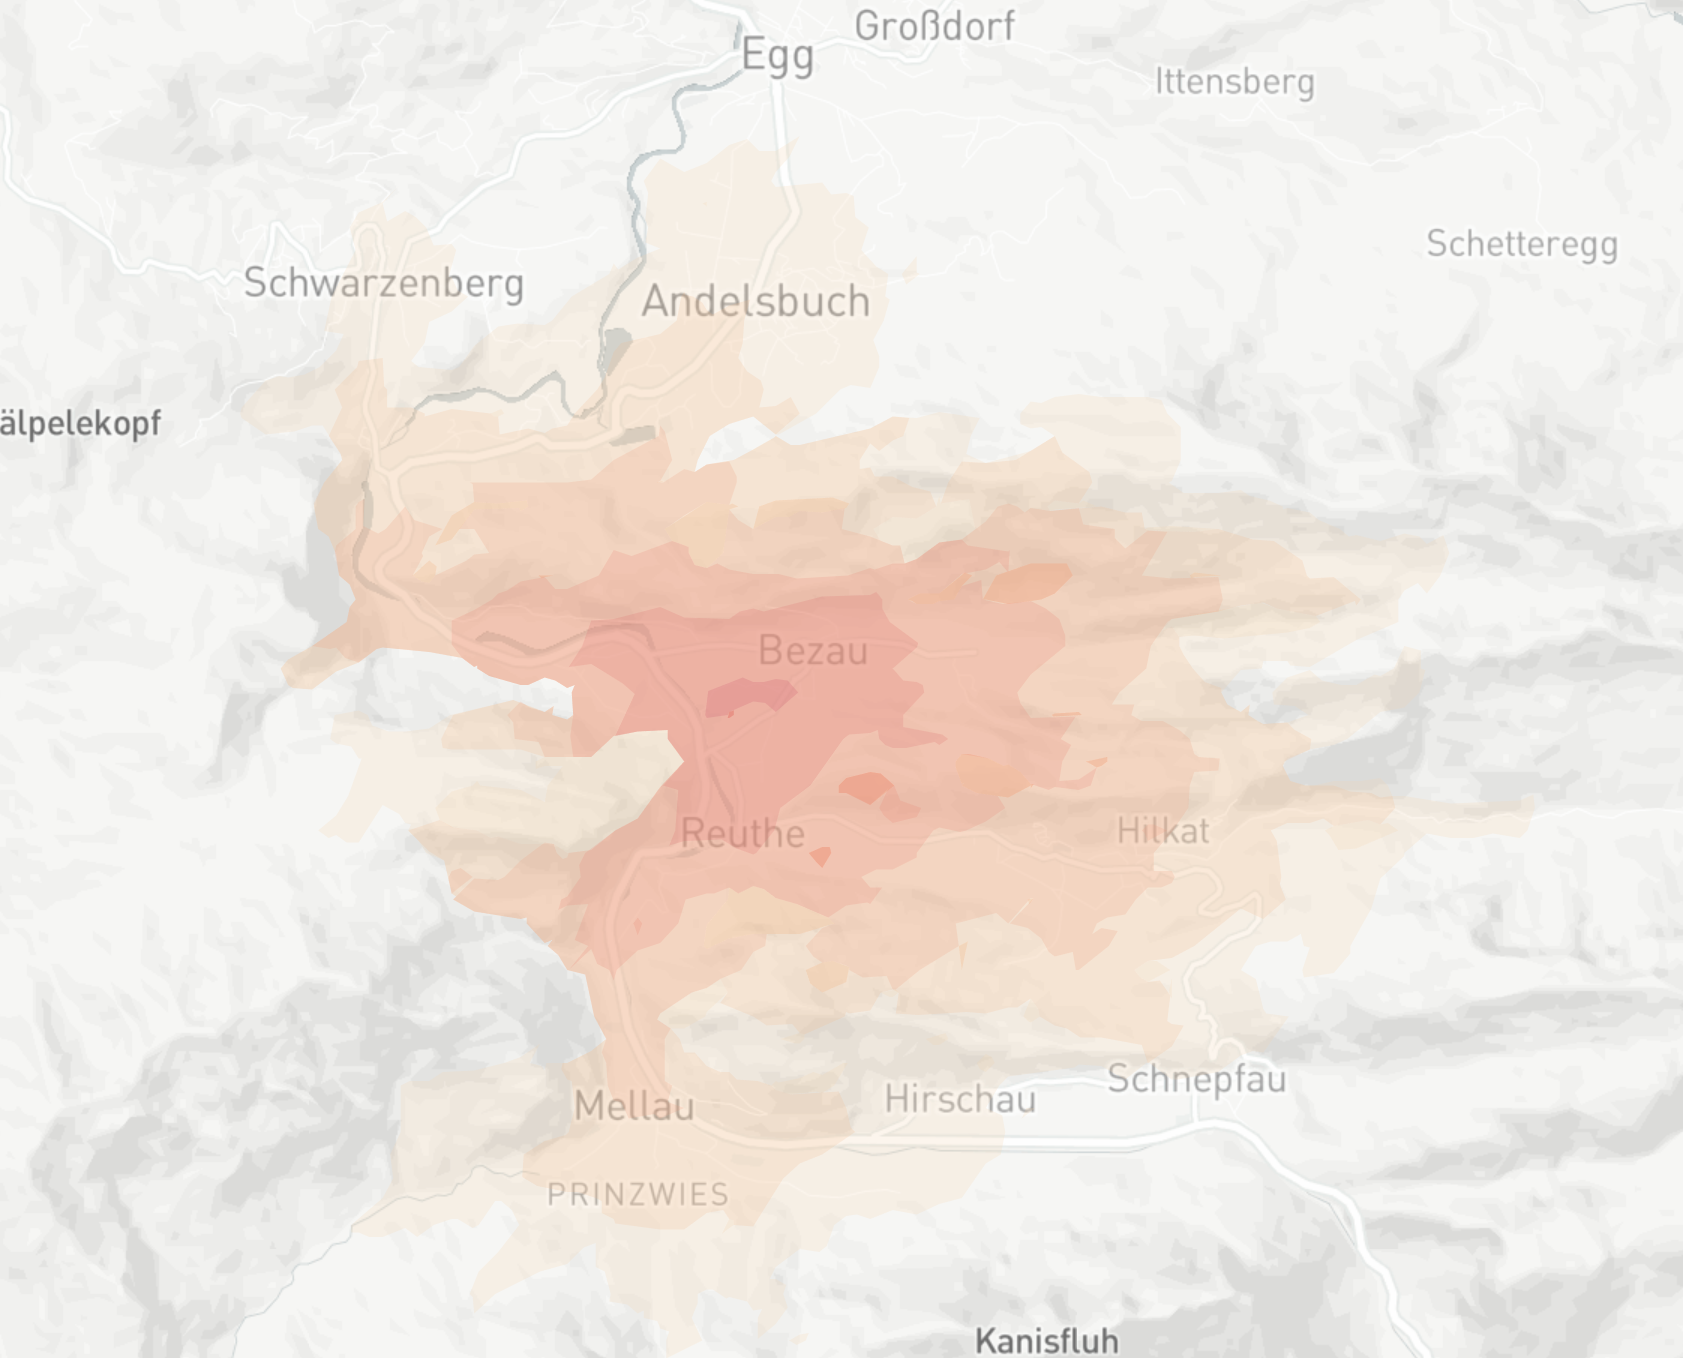
\includegraphics[scale=.6]{pics/color-scheme-example}
    \caption{Color Scheme Beispiel: Je heller die Farbe, desto länger dauert die Anreise mit dem Fahrrad in die Mitte}
    \label{fig:color-scheme-example}
\end{figure}

\subsection{Sidebar}
Die Sidebar auf der linken Seite bietet Platz, um Informationen anzuzeigen.
Ganz oben ist der \emph{title} zu sehen, darunter der \emph{subtitle}, der zu sehende Textblock, ist die \emph{description},
für welche für jeden Array Eintrag ein eigener Absatz erstellt wird.
Am unterende Ende der Sidebar sind die Filter angeordnet, standardmäßig für jede Data Source wird ein Sichtbarkeits-Filter angelegt,
mit diesem lässt sich die Data Source ein- oder ausblenden.
Der zweite unterstütze Filter ist der "Slider", mit diesem kann man den Wertebereich der angezeigten Daten verändern,
zum Beispiel, wenn man nur die Daten zwischen einer Anreise Dauer von 800 Sekunden bis 1000 Sekunden angezeigt haben möchte, kann man dies hier machen.
Gelöst wird das ganze mit einem Value-Binding auf das Attribut, welches in der Konfiguration angegeben wird, auch
die Skalierung des Slider wird automatisch berechnet.

\begin{figure}[hbt!]
    \centering
    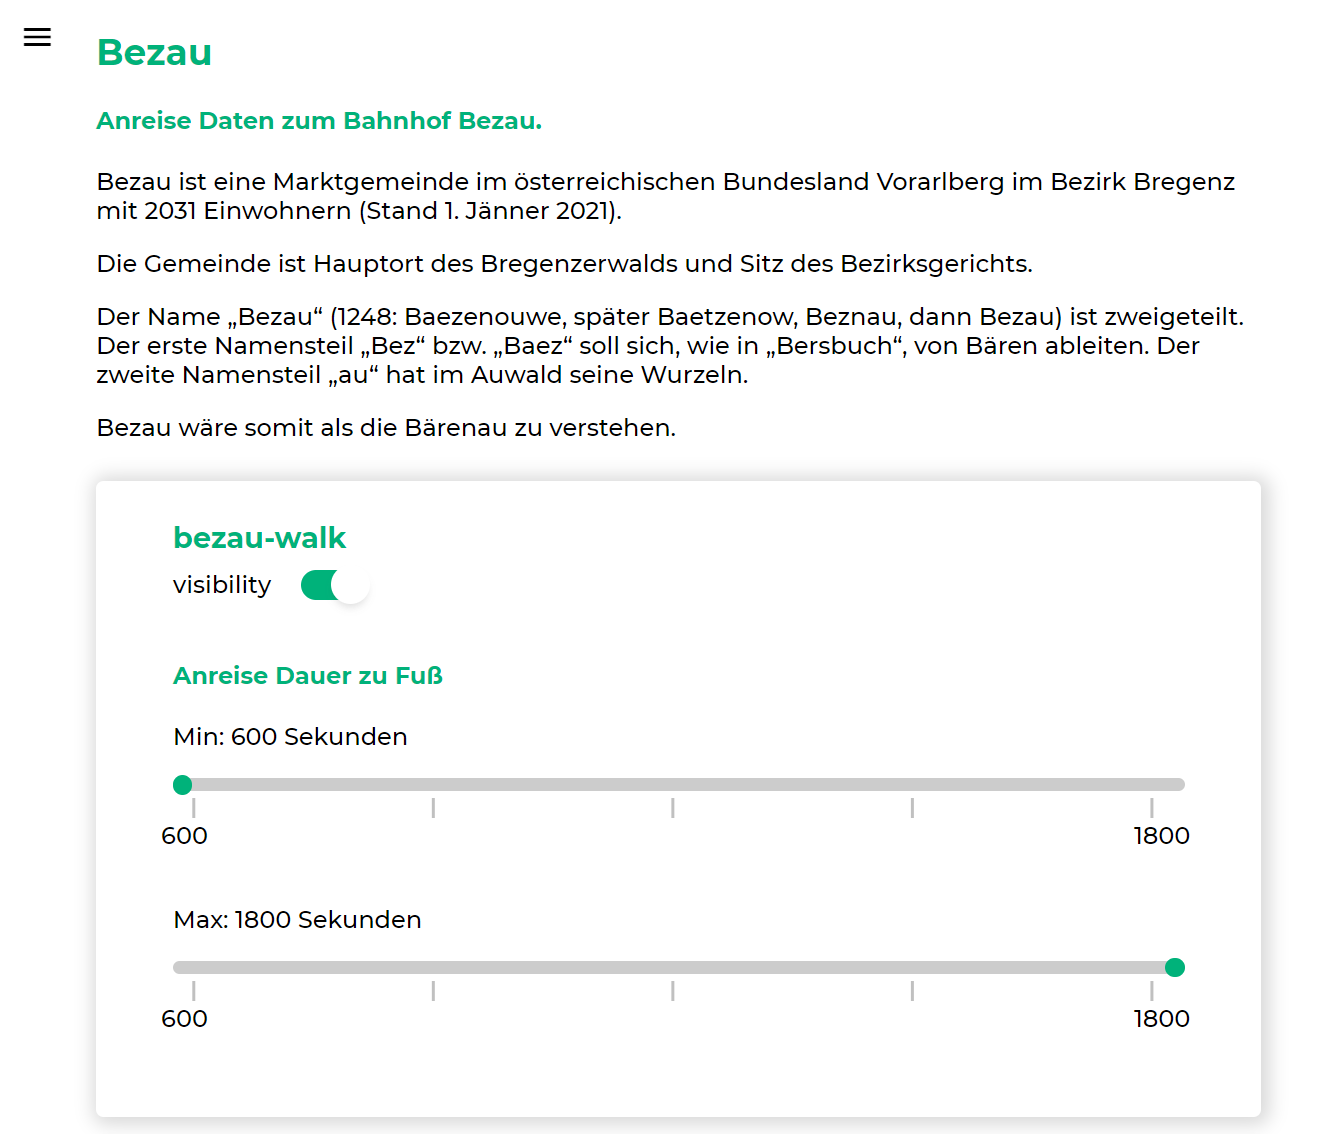
\includegraphics[scale=.7]{pics/sidebar}
    \caption{Sidebar mit Beispiel Daten}
    \label{fig:sidebar}
\end{figure}

\subsection{Map}
In der Map werden alle Daten auf der Karte visualisiert.
In den hochgeladenen Geo-JSON Files sind unzählige Koordinaten enthalten, welche Punkteweise auf der Karte dargestellt werden,
je nach Art der Darstellung, werden anschließend Linien zwischen Punkten berechnet, welche auch Formen ergeben können.
Die Arten dieser Visualisierungen sind im RFC 7946~\cite{rfc7946} Standard genau beschrieben, diese werden auch bei webmap angewandt.

Durch den Data Source Service, gibt es bereits eine Sammlung an LayerGroups, welche nur noch angezeigt werden müssen,
dass erhöht nicht nur die Performance, wenn die Page gewechselt wird, sondern macht die gesamte Applikation gut strukturiert.

Wenn alle Components eingebunden sind, kann das Frontend so ausschauen:
\begin{figure}[hbt!]
    \centering
    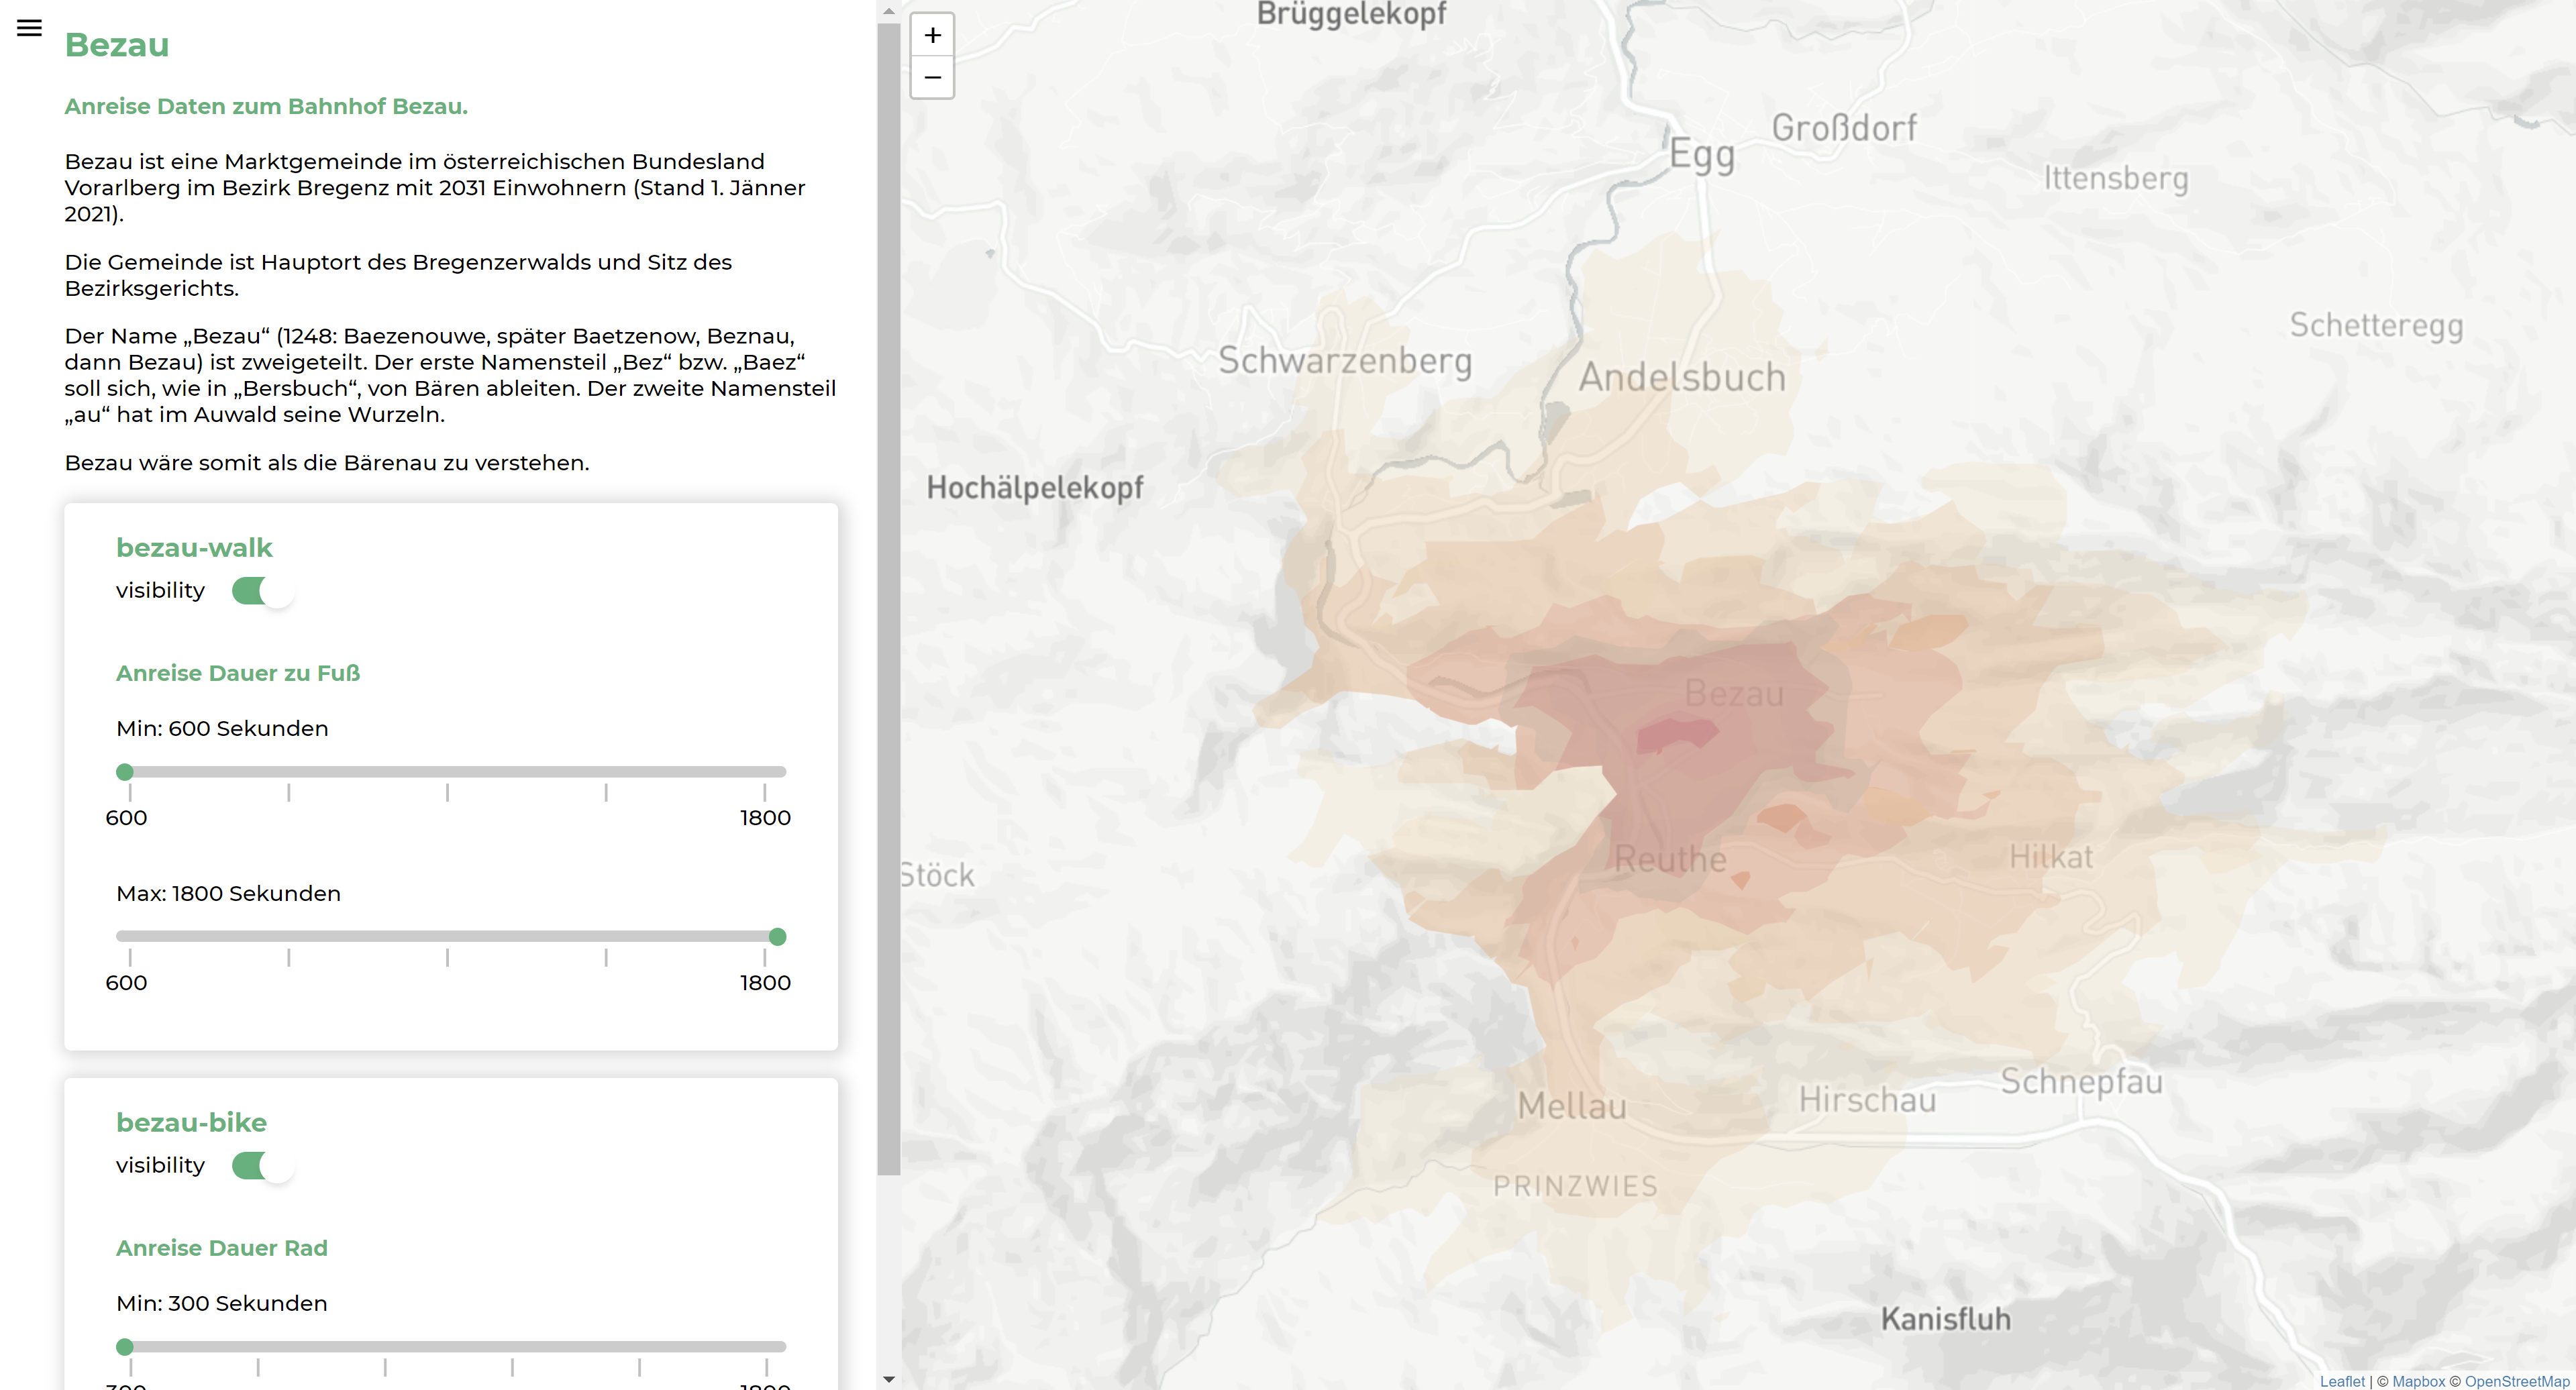
\includegraphics[scale=.3]{pics/webmap-frontend}
    \caption{Webmap Frontend}
    \label{fig:webmap-frontend}
\end{figure}


\section{Generator Implementierung}
\setauthor{Sebastian Scholl}
Der Generator soll dazu dienen, ein Konfigurationsfile bzw. ein Angular Projekt basierend auf diesem Konfigurationsfile
schnell und einfach in einer Benutzeroberfläche zu erstellen.


\subsection{JSON Schema}
Da der Generator dynamisch aufgebaut sein sollte und die Möglichkeit bestehen sollte, das Format der generierten
Daten zu verändern, wurde sich dazu entschieden, den Generator aufgrund eines JSON Schemas, das die Daten beschreibt,
aufzubauen.

Das Format des Schemas wurde daher so angepasst, dass es die benötigten Daten möglichst genau beschreiben kann.

Jede Property hat ein \textit{type} und \textit{description} Feld.
\textit{type} ist erforderlich, während \textit{description} optional ist.
Der Wert von \textit{type} kann einer der folgenden Strings sein:

\begin{itemize}
  \item "object"
  \item "array"
  \item "string"
  \item "number"
  \item "boolean"
  \item "file"
\end{itemize}

Ist die Property ein Object, hat es die Felder \textit{properties} und \textit{required}, die beide optional sind.
\textit{properties} ist ein Object mit den Namen der Properties des zu beschreibenden Objects als Keys.
Der Wert ist dabei wiederrum eine Property.
Werden keine Properties definiert, kann im Generator an dieser Stelle ein beliebiges JSON-Object eingegeben werden.
\textit{required} ist ein Array mit den Namen der Properties, die erforderlich sind.

Ist die Property ein Array, hat es zusätzlich das erforderliche \textit{items} Feld.
Der Wert beschreibt die Properties, die sich in diesem Array befinden.
Im Gegensatz zur offiziellen Definition des JSON-Schemas kann hier nur \textit{eine} Property definiert werden.

Properties vom Typ "number" können optional die Felder \textit{minimum} und \textit{maximum} enthalten.

Properties, die den Typ "file" haben, können im optionalen Feld \textit{fileExtensions} die erlaubten
Dateiendungen als Array definieren.
Im Generator wird an dieser Stelle ein File-Upload angezeigt.

Properties vom Typ "string" und "boolean" haben keine zusätzlichen Felder.

\section{Angular Projekt}
Da sich reaktive Formulare einfach in Angular umsetzen lassen, wurde sich für dieses Framework entschieden.
Ein weiterer Vorteil ist, dass damit der Generator und das Frontend beide in Angular umgesetzt sind, was die
Wartung des gesamten Projekts erleichtert.

Das Kernstück des Generators ist das \textit{src/assets/schema.json} File, in dem sich das Schema für das zu
generierende Konfigurationsfile befindet.
Aufgrund dessen werden Input-Felder generiert, in welchen Benutzer und Benutzerinnen die entsprechende
Konfiguration eingeben können.

Für jeden Typ, den eine Property haben kann wurde eine Angular-Komponente definiert.
Weiters wurde mit sogenannten \textit{FormControl} Objekten der Inhalt der Input-Felder auf die im Schema definierten
Kriterien überprüft.
So kann man zu jeder Zeit einfach überprüfen, ob alle eingegebenen Werte valide sind.

Beim Laden der Seite wird also für jede Property, die im Schema definiert ist, eine entsprechende Komponente generiert.
Beim Klick auf einen Button werden dann alle Werte, die in die Komponenten eingegeben wurden, in ein entsprechendes
JSON-Objekt gespeichert, welches dann als Konfigurationsdatei an das Backend gesendet wird.

Um den Fokus auf die Funktionalität legen zu können, wurde für das Design \textit{Angular Material} verwendet.

\subsection{Object Component}
Ein Object Component dient lediglich zur Visualisierung, welche Properties zu welchem Objekt gehören.
Die Funktionalität befindet sich hauptsächlich in den anderen Komponenten.

Eine Ausnahme bildet ein Objekt, bei dem im Schema keine \textit{properties} definiert sind.
In diesem Fall wird ein Textfeld angezeigt, in welches ein beliebiges JSON-Objekt eingegeben werden kann.
Mittels \textit{FormControl} wird laufend überprüft, ob der eingegebene Wert ein valides JSON-Objekt ist.

\subsection{Array Component}
Ein Array Component listet alle Werte, die sich in diesem Array befinden, auf.
Mit einem Button kann ein neuer Wert hinzugefügt werden.

\subsection{File Component}
Bei einem File Component wird ein Button zum Uploaden von Files angezeigt.
Ein \textit{FormControl} Objekt überprüft bei einem Upload, ob die Dateiendung mit den im Schema definierten
Endungen übereinstimmt.

\subsection{Number Component}
Ein Number Component besteht aus einem einfachen Input-Feld, in das nur Zahlen eingegeben werden.
Dabei wird auch das im Schema definierte \textit{minimum} und \textit{maximum} überprüft.

\subsection{String Component}
Der String Component wird durch ein Input-Feld dargestellt, in das beliebige Zeichen eingegeben werden können.

\subsection{Boolean Component}
Der Boolean Component wurde mit einem Schieberegler realisiert, der zwei Zustände annehmen kann: \textit{true} und
\textit{false}.

\subsection{Generieren des Konfigurationsfiles}
Mit einem Klick auf den Button \textit{Download config.json} kann die Konfigurationsdatei heruntergeladen werden.
Klickt man auf \textit{Create project} wird diese Konfigurationsdatei, sowie alle weiteren hochgeladenen Dateien, an
das Backend gesendet und man erhält das daraus generierte Projekt.

\begin{lstlisting}[numbers=left]
{
  "title": "Example JSON Object",
  "type": "object",
  "properties": {
    "string": {
      "type": "string"
    },
    "number": {
      "type": "number"
    },
    "boolean": {
      "type": "boolean"
    },
    "array": {
      "type": "array",
      "items": {
        "type": "string"
      }
    },
    "object": {
      "type": "object",
      "properties": {
        "another string": {
          "type": "string"
        },
        "another number": {
          "type": "number"
        }
      }
    }
  }
}
\end{lstlisting}

Folgende Seite wird aufgrund obigem JSON-Schema angezeigt:

\begin{figure}[hbt!]
  \centering
  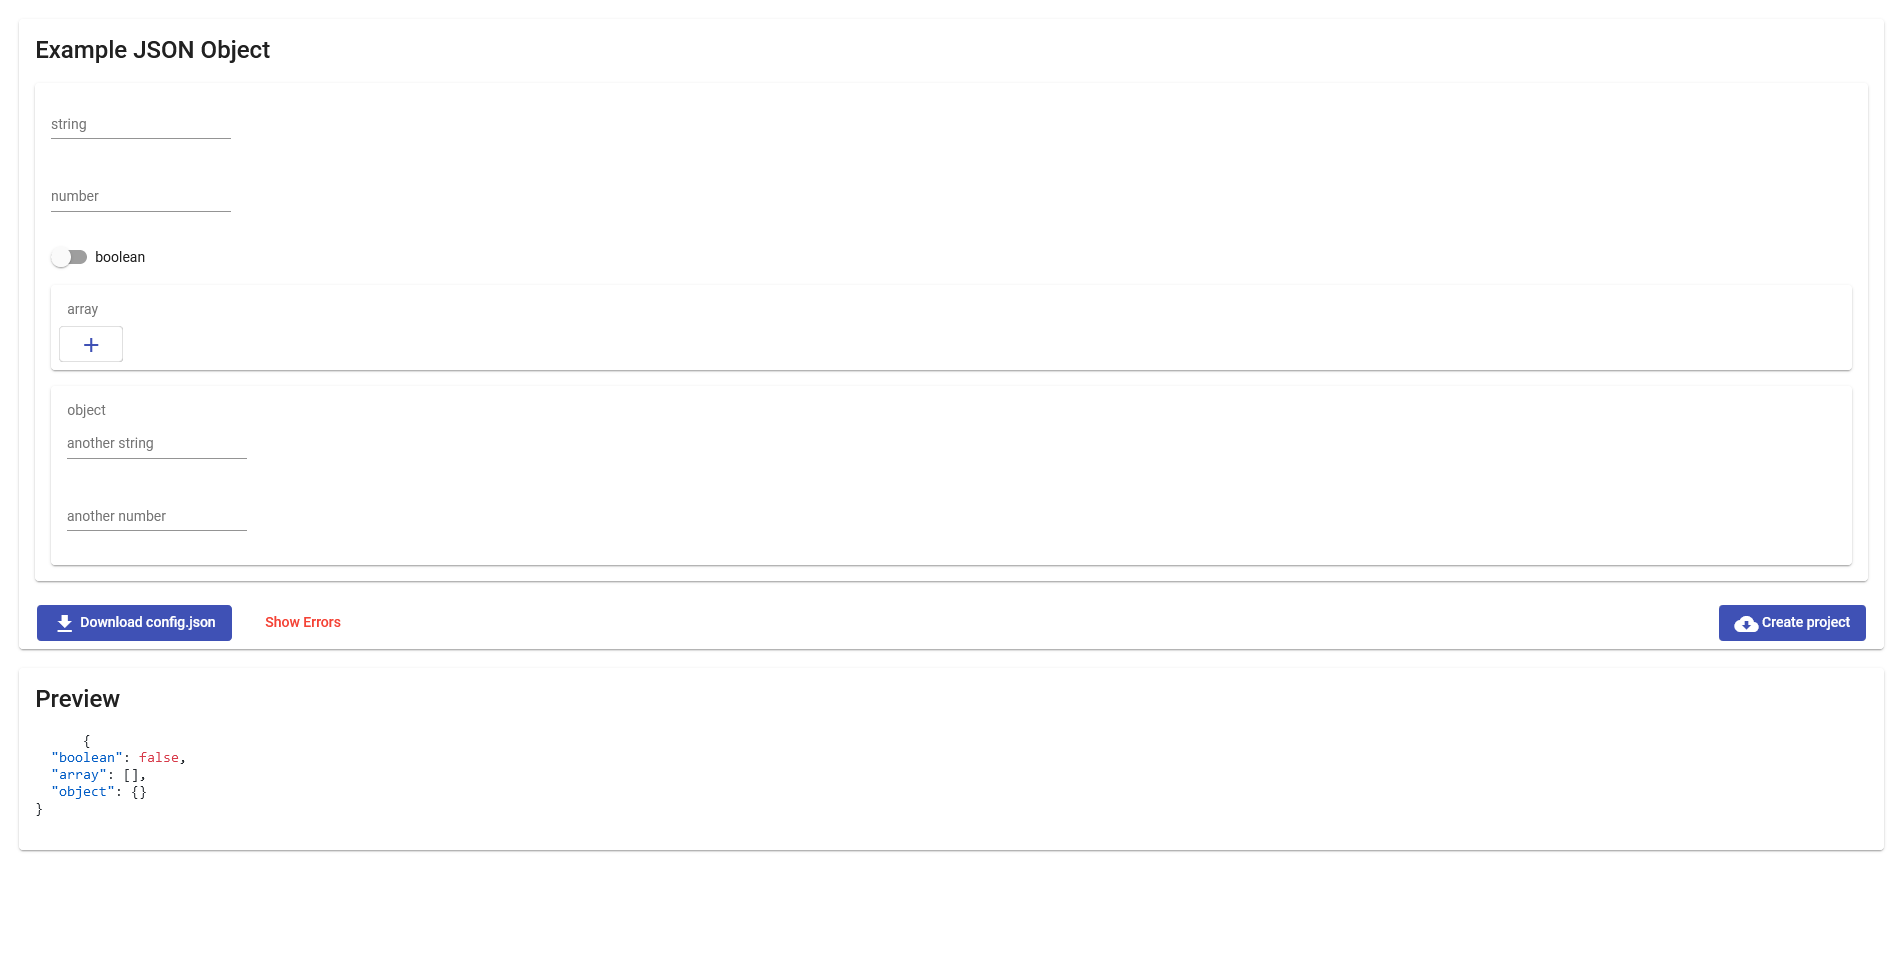
\includegraphics[scale=.2]{pics/generator}
  \caption{Generator}
\end{figure}


\section{Backend Implementierung}
\setauthor{Sebastian Scholl}

\subsection{Static Site Generators}
Da JSON als Format für die Daten ausgewählt wurde und Angular dieses zur Laufzeit einlesen kann, wurden
keine Static Site Generators zum Generieren der Websites verwendet.

\subsection{Aufbau}
Das Backend besteht aus zwei Teilen, die verschiedene Aufgaben übernehmen:

\begin{itemize}
    \item Eine REST-API für das Generieren eines Angular-Projekts aufgrund der im Generator erstellten Konfiguration
    \item Das Hosten des Generators
\end{itemize}

\subsubsection{REST-API}
Die API wurde in TypeScript geschrieben und läuft in der Laufzeitumgebung Node.js.
Für die Implementierung der Endpoints wurde express.js verwendet.

Das Template-Angular-Projekt, aus dem später mithilfe einer Konfigurationsdatei das Projekt generiert wird,
befindet sich im \textit{template} Directory.
Beim Start wird mithilfe des Node-Packages \textit{node-tar} daraus das Archiv \textit{template.tar} erzeugt.

Die API enthält drei Endpoints:

\begin{itemize}
    \item GET /api/status
    \item GET /api/configuration/:filename
    \item POST /api/configuration
\end{itemize}

\paragraph{GET /api/status}
Der Endpoint dient zur Überprüfung, ob die API erreichbar ist.
Er sendet in diesem Fall \textit{Server is running} als Response.

\paragraph{GET /api/configuration/:filename}
Dieser Endpoint dient zum Download der generierten Projekte.
Der Parameter \textit{filename} ist dabei der Name einer \textit{.tar.gz}-Datei, die sich im \textit{public}
Directory befindet.

\paragraph{POST /api/configuration}
Ein Request zum diesem Endpoint enthält einen Request-Body des Typs
\textit{multipart/form-data}.
Darin sind die Konfigurationsdatei für das zu generierende Projekt, sowie alle weiteren benötigten Files enthalten.

Zuerst wird ein temporäres Directory im Pfad für temporäre Dateien des jeweiligen Betriebssystems erstellt.
Darin werden alle gesendeten Files gespeichert.
Da das Directory mit der Methode \textit{mkdtemp} des Node-Packages \textit{fs} erstellt wird, erhält es einen
zufälligen und eindeutigen Namen.
Dadurch können mehrere Requests zur gleichen Zeit abgewickelt werden.
Danach wird eine Kopie des \textit{template.tar} Archives in diesem Directory erstellt.
Zu diesem werden die gesendeten Files hinzugefügt und es wird anschließend mit \textit{gzip} komprimiert.
Das entstandene File wird dann in das \textit{public} Directory kopiert und das temporäre Directory wird wieder gelöscht.

Waren alle diese Schritte erfolgreich, wird ein Response mit dem HTTP Status 201 (Created)
gesendet.
Der Response-Header \textit{Location} enthält dabei die URL zum Download des generierten Projekts.
Nach 10 Minuten läuft dieser Downloadlink ab und das generierte Projekt wird gelöscht.

\subsubsection{Webserver}
Als Webserver und Reverse-Proxy wird nginx verwendet.
Der Webserver stellt alle Files des Generators, die sich im \textit{/usr/share/nginx/html/generator} Directory
befinden, zur Verfügung, während der Reverse-Proxy alle Requests zu \textit{/api} zur REST-API weiterleitet.
Dieser läuft am Port 4000.

Die Konfigurationsdatei dafür sieht folgendermaßen aus:

\begin{lstlisting}[numbers=left]
  events {}

  http {
    include mime.types;

    server {
      location /api {
        proxy_pass http://server:4000/api/;
      }

      location / {
        root /usr/share/nginx/html/generator;
      }
    }
  }
\end{lstlisting}

\subsection{Containerization}
Da beide Teile des Backends verschiedene Aufgaben übernehmen lag es nahe, dieses in der Microservice
Architektur umzusetzen.
Daher laufen die beiden Teile in unterschiedlichen Docker Containern und werden mithilfe
von Docker Compose orchestriert.

Die Images dafür werden in \textit{Dockerfiles} definiert.

Das \textit{docker-compose.yml} File sieht folgendermaßen aus:

\begin{lstlisting}[numbers=left]
  version: '3.8'

  services:
    nginx:
      build: .
      ports:
        - 80:80
      restart: always
      volumes:
        - ./nginx:/etc/nginx:ro

    server:
      build: server
      restart: always
      environment:
        NODE_PORT: 4000
        NODE_ENV: production
        TEMPLATE_DIR: template
        PUBLIC_DIR: public
      volumes:
        - ./server:/usr/src/app
        - /usr/src/app/node_modules
        - /usr/src/app/dist
\end{lstlisting}

Das gesamte Backend kann somit mit dem Befehl \textit{docker-compose up -d} gestartet werden.

\subsubsection{Webserver Image}
Das Image für den Webserver und Reverse Proxy macht sich sogenannte Multi-Stage-Builds zunutze.
Dabei werden mehrere Base Images angegeben.
Das kann beispielweise genutzt werden, um die Applikation in einem Base Image zu builden und in einem anderen
zu starten.

Im Fall des Webservers wird zuerst das \textit{node} Image verwendet, um den Generator zu kompilieren.
Die entstehenden Files werden dann in das \textit{nginx} Image kopiert, wo sie vom Webserver bereitgestellt werden.

Das \textit{Dockerfile} dazu sieht folgendermaßen aus:

\begin{lstlisting}[numbers=left]
FROM node:16-alpine AS builder
WORKDIR /usr/src/app
COPY client/package*.json ./
RUN npm install
COPY client/ ./
RUN npm run lint \
    && npm run build

FROM nginx:1.21.1-alpine
COPY --from=builder /usr/src/app/dist /usr/share/nginx/html
\end{lstlisting}

\subsubsection{REST-API Image}
Im Dockerfile der REST-API werden folgende Schritte ausgeführt:

\begin{itemize}
  \item Das Base Image \textit{node} wird verwendet
  \item \textit{/usr/src/app} wird als das Directory festgelegt, in dem alle folgenden Befehle ausgeführt werden
  \item \textit{package.json} und \textit{package-lock.json} werden in das Image kopiert
  \item Dependencies werden mit \textit{npm install} installiert
  \item Alle weiteren Files aus dem Directory, in dem sich das \textit{Dockerfile} befindet, werden in das Image kopiert
  \item Das Projekt wird gelintet und gebuildet
  \item \textit{npm start} wird als Befehl definiert, der beim Start eines Containers ausgeführt wird
\end{itemize}

Das entsprechende \textit{Dockerfile} sieht wie folgt aus:

\begin{lstlisting}[numbers=left]
FROM node:16-alpine

WORKDIR /usr/src/app

COPY package*.json ./

RUN npm install

COPY . .

RUN npm run lint \
    && npm run build

CMD [ "npm", "start" ]
\end{lstlisting}

\section{Deployment Pipeline}
\setauthor{Sebastian Scholl}
Mit der Deployment Pipeline sollen Benutzern und Benutzerinnen die Möglichkeit haben, das generierte Projekt schnell
und einfach zu deployen.
Das Ziel des Deployments ist dabei entweder eine Linux Virtual Machine oder eine Firebase Hosting Instanz.

\subsection{Jenkins}
Um das Projekt mit Jenkins deployen zu können, wurden zwei Files erstellt: \textit{Jenkinsfile.ssh} und
\textit{Jenkinsfile.firebase}.
Je nach Ziel des Deployments konnte eines der beiden beim Erstellen der Pipeline im Web-Interface von Jenkins
angegeben werden.

Um die Dateien zur Virtuellen Maschine zu senden, wurde das Jenkins-Plugin \textit{Publish Over SSH}
verwendet.
Für das Deployen zu \textit{Firebase Hosting} stand kein Plugin zur Verfügung.
Stattdessen wurde auf die \textit{Firebase CLI} zurückgegriffen.

Die SSH-Konfiguration der Virtuellen Maschine musste dabei nur einmal in Jenkins vorgenommen werden und konnte
dann in jeder Pipeline verwendet werden.
Auch für Firebase musste nur einmalig ein Token generiert werden, mit dem man sich dann in jeder Pipeline
authentifizieren konnte.

Ein großer Nachteil von Jenkins war jedoch, dass für jedes Projekt zuerst ein GitHub
Repository und eine neue Pipeline im Web-Interface von Jenkins erstellt werden
musste, bevor es automatisch deployed werden konnte.

\subsection{GitHub Actions}
Für den Ansatz mit GitHub Actions wurden die beiden Files \textit{deploy.yml} und \textit{firebase.yml} im
\textit{.github/workflows} Directory des Projekts erstellt.

Sowohl für das Deployen auf eine Virtual Machine, als auch zu \textit{Firebase Hosting}
standen Plugins zur Verfügung, was die Konfiguration einfacher als bei Jenkins machte.
Hostname, Username, Target Direcory und SSH Private Key der Virtual Machine und Informationen zur Firebase Instanz
wurden als Secrets gespeichert und so in den Workflows verwendet.

Wie auch bei einer Jenkins Pipeline musste für jedes Projekt jedoch auch beim
Ansatz mit GitHub Actions ein GitHub Repository erstellt werden.

\subsection{Node.js Skripts}
Da für ein Deployment mithilfe von Skripts kein GitHub Repository für jedes Projekt erstellt werden muss,
wurde sich für diesen Ansatz entschieden.
Um das gesamte Projekt leichter wartbar zu machen wurden auch die Deployment Skripts in JavaScript geschrieben.
Diese werden über den Package Manager \textit{npm} mit \textit{npm run deploy:ssh} bzw.
\textit{npm run deploy:firebase} aufgerufen.
Diese Befehle werden im \textit{package.json} File definiert:

\begin{lstlisting}[numbers=left]
{
  "name": "webmap",
  "version": "0.0.0",
  "scripts": {
    ...
    "deploy:firebase": "node deploy/firebase.js",
    "deploy:ssh": "node deploy/ssh.js"
  },
  ...
}
\end{lstlisting}

\subsubsection{Firebase Skript}
Das Firebase Skript führt folgende Schritte aus:

\begin{itemize}
    \item Installieren der Dependencies
    \item Linten des Projekts
    \item Builden des Projekts
    \item Deployen mithilfe der Firebase CLI
\end{itemize}

Um die jeweiligen Konsolenbefehle in Node.js aufzurufen wurde die Methode \textit{spawn} des Node-Packages
\textit{child\_process} verwendet.
Dieses wird standardmäßig mit Node.js mitgeliefert und benötigt daher keine zusätzliche Installation.

Bevor zu Firebase deployed werden kann, muss der Benutzer oder die Benutzerin die Project ID des jeweiligen
Firebase Projekts eingeben.
Dieses wird im \textit{.firebaserc} File gespeichert, das dann von der Firebase CLI ausgelesen wird.

Die Firebase CLI besteht aus einer ausführbaren Datei, die sich im \textit{node\_modules/.bin} Directory befindet.
Der Name dieser Datei unterscheidet sich auf Windows jedoch von der auf anderen Betriebssystemen.
Daher musste beim Aufrufen der CLI überprüft werden, auf welchem Betriebssystem das Skript ausgeführt wird.
Diese Information stellt Node.js in der Variable \textit{process.platform} bereit.

\subsubsection{SSH Skript}
Das SSH Skript unterscheidet sich vom Firebase Skript nur im letzten Schritt.
In diesem wird das Node-Package \textit{node-ssh} verwendet, um das gebuildete Projekt zu deployen.

Auch hier werden wieder Informationen, die für das Deployment benötigt werden, von Benutzer oder Benutzerin über
die Kommandozeile eingelesen.
Diese werden im \textit{ssh-config.json} File gespeichert.
